\documentclass[a4paper]{article}
\title{Sweave Example 1} 
\author{Friedrich Leisch}
\usepackage{Sweave} 
\begin{document}
\Sconcordance{concordance:test.tex:test.Rnw:%
1 9 1 1 2 1 0 2 1 9 0 1 2 2 1 1 2 1 0 1 1 4 0 1 2 1 1}

\maketitle
In this example we embed parts of the examples from the 
\texttt{kruskal.test} help page into a \LaTeX{} document:

\begin{Schunk}
\begin{Sinput}
> data(airquality , package="datasets")
> library ("stats")
> kruskal.test(Ozone ~ Month, data = airquality) 
\end{Sinput}
\begin{Soutput}
	Kruskal-Wallis rank sum test

data:  Ozone by Month
Kruskal-Wallis chi-squared = 29.3, df = 4, p-value = 6.901e-06
\end{Soutput}
\end{Schunk}

which shows that the location parameter of the Ozone distribution varies significantly from month to month. Finally we include a boxplot of the data:
\begin{center}
\begin{Schunk}
\begin{Sinput}
> library ("graphics")
> boxplot(Ozone ~ Month, data = airquality) 
\end{Sinput}
\end{Schunk}
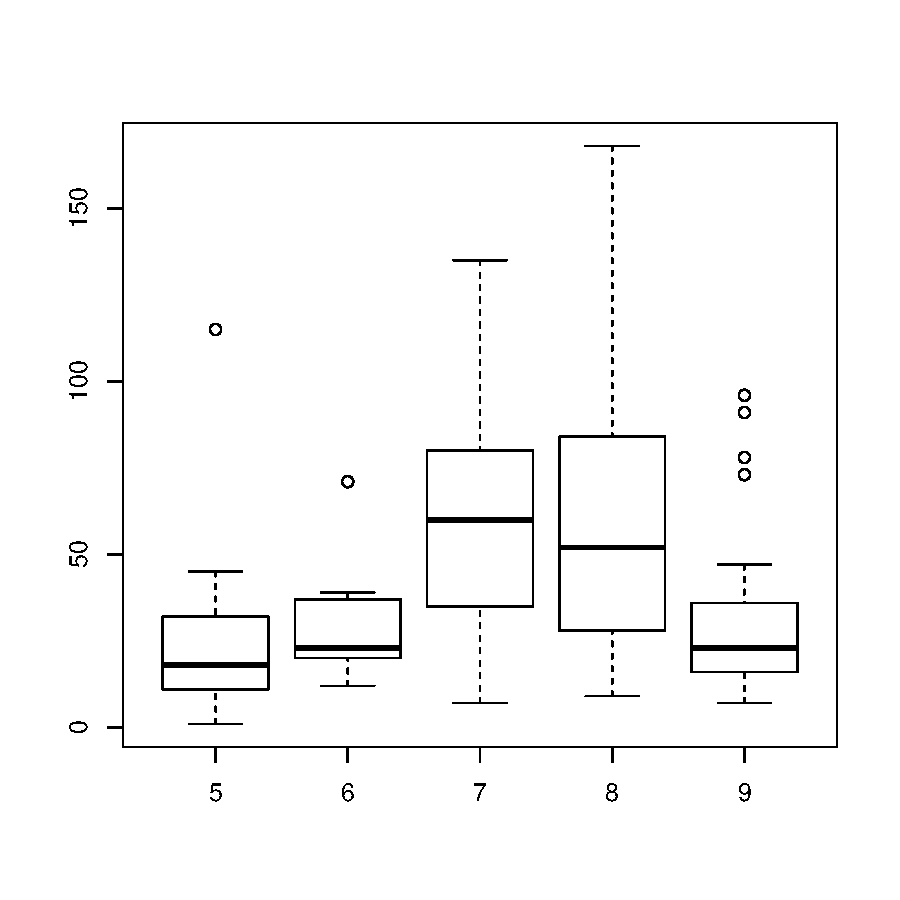
\includegraphics{test-002}
\end{center}
\end{document} 
